\documentclass{beamer}

\usetheme{Antibes}
\usecolortheme{rose}

\usepackage[utf8]{inputenc}
\usepackage[russian]{babel}
\usepackage{graphicx} 
\usepackage{epstopdf}
\usepackage{tikz}
\usepackage[overlay]{textpos}
\usepackage{color}

\setbeamertemplate{caption}{\insertcaption}

%%% Math commands %%%
\DeclareMathOperator*{\argmin}{\arg\!\min}
\DeclareMathOperator*{\argmax}{\arg\!\max}

\newcommand{\tikzmark}[2][minimum width=3cm,minimum height=0.7cm]{
 \tikz[remember picture,overlay]
 \node[anchor=south west,
       inner sep=0pt,
       outer sep=0pt,
       xshift=0em,
       yshift=-3ex,
       #1](#2){};
}

\newcommand{\shownode}[1]{
  \tikz[remember picture,overlay]\draw[red](#1.south east)rectangle(#1.north west);
}

\newcommand{\mathp}[2]{\mathbf{P}(#1| #2)}
\newcommand{\myexp}[1]{\exp(#1)}
\newcommand{\mathe}[2]{\mathbf{E}(#1| #2)}
\newcommand{\mathee}[1]{\mathbf{E}(#1)}
\newcommand{\mathpwave}[2]{\tilde{\mathbf{P}}(#1| #2)}
\newcommand{\grad}[2]{\frac{\partial #1}{\partial #2}}
\newcommand{\gradp}[3]{\frac{\partial \log \mathp{#1}{#2}}{\partial #3}}

    \setbeamertemplate{footline}[page number]
      
%\logo{
\includegraphics[height=0.7cm]{picture/msu.pdf}}
\title{Модификации метода стохастического градиентного спуска для задач машинного обучения с большими объемами данных}
\author[Chabanenko]{Владислав Чабаненко\\[5mm]Научный руководитель: к.ф-м.н., доцент \\Ветров Дмитрий Петрович}
\institute[ВМК МГУ имени М.В. Ломоносова]
{
\medskip
}
\date{2016}

\begin{document}

\begin{frame}
	\titlepage
\end{frame}

\section{Теория}

\begin{frame}
	\frametitle{Обучение нейронных сетей}
Проблема:
\begin{itemize}
\item Медленная сходимость из-за изменения распределений на слоях в процессе обучения
%\item Существующие подходы задействуют весь объем выборки %проблема памяти, подходы --- PCA?
\end{itemize}	
	
Решение --- батч-нормализация (БН) \footnote{http://arxiv.org/abs/1502.03167}:
\begin{itemize}
\item Подсчет необходимых статистик в слое по батчам (эмпирические средние и дисперсии) %решена проблема памяти
\item Нормализация распределения на каждом слое нейронной сети с помощью подсчитанных статистик %ускоряет обучение сети
\end{itemize}
	
\end{frame}

	
%	Не так давно (в феврале 2015 года) была опубликована статья по применению батч-нормализации к нейронным сетям с целью ускорения их обучения. Идея метода: распределение на каждом слое нейронной сети меняется в процессе обучения, что замедляет обучение --- авторы предлагают выравнивать распределения на каждом слое с помощью нормализации --- приведения выхода слоя к нормальному распределению. В результате для каждого слоя исходной нейронной сети мы вычисляем необходимые статистики (эмпирическое матожидание и дисперсию) по батчам и на выходе получаем с помощью нехитрых преобразований (вычитание матожидание и деление на корень из дисперсии) слой с примерно нормальным распределением. Активно используется по всему миру, встроен в библиотеки (lasagne, tensorflow).

\begin{frame}
\frametitle{Актуальность батч-нормализации}

\begin{itemize}
\item Батч-нормализация сейчас очень популярна, так как многие state-of-the-art архитектуры сетей без нее совсем плохо обучаются
\item Работает при больших объемах данных, что в сейчас очень актуально
\end{itemize}
\end{frame}
	

\begin{frame}
\frametitle{Применение батч-нормализации}
\begin{itemize}
%\item После каждого слоя исходной сети добавляется дополнительный БН-слой
\item Авторы идеи применили БН для метода стохастического градиентного спуска (SGD)
\item Мы исследовали применение БН к различным популярным модификациям SGD, используемых при обучении нейронных сетей
\end{itemize}
\end{frame}
	
	

\begin{frame}
\frametitle{Модификации SGD}	
	
В работе рассматривались следующие модификации SGD:

\begin{itemize}
\item SGD с инерцией (SGDm) %учитываем с некоторым весом градиент на предыдущей итерации
\item Adagrad %перемасштабируем вес каждого элемента градиента с учетом величины суммы квадратов прошлых градиентов
\item RMSprop %то же самое, что Адаград, только поддерживается экспоненциальное скользящее среднее прошлых градиентов -- оценка второго момента градиента
\item Adadelta %работает, как RMSprop, но добавлен хитрый моментум
\item Adam %точно такой же, как RMSprop, только добавлен моментум в числитель шага
\end{itemize}

\end{frame}

\begin{frame}
\frametitle{Интуиция методов}
\begin{figure}
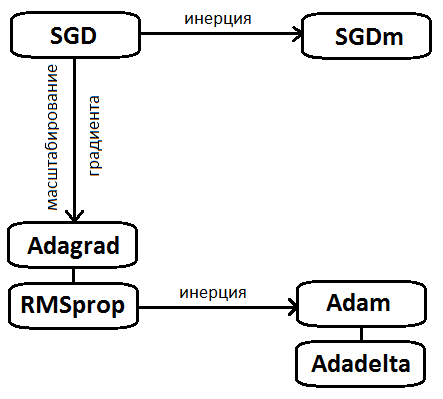
\includegraphics[scale=0.5]{methods.png}
\end{figure}
\end{frame}



\section{Эксперименты}

\begin{frame} 
\frametitle{Датасеты}	
В рамках работы мы проводили экспериментальные исследования на следующих датасетах:
\begin{itemize}
\item MNIST (70 тыс. рукописных цифр --- 10 классов)
\item CIFAR-10 (60 тыс. изображений --- 10 классов)
\end{itemize}	

\begin{minipage}{0.45\linewidth}
\begin{figure}
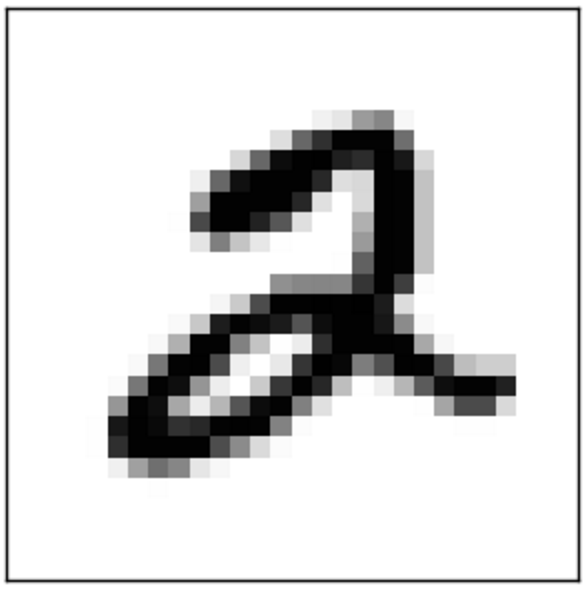
\includegraphics[scale=0.3]{mnist_img.png}
\end{figure}
\end{minipage} \hfill
\begin{minipage}{0.45\linewidth}
\begin{figure}

\includegraphics[scale=0.4]{cifar_img.jpeg}
\end{figure}
\end{minipage}

\end{frame}

\begin{frame}
\frametitle{Архитектуры}
Использовались следующие архитектуры:
\begin{itemize}
\item Полносвязная сеть с 3 скрытыми слоями по 100 нейронов (MLP)
\item Сеть с двумя сверточными слоями (32 фильтра $5 \times 5$ + макс-пулинг с окном $2\times 2$) и один полносвзяный слой c 256 нейронами (CNN)
\end{itemize}	

Для обеих архитектур использовалась функция активации ReLU.
\end{frame}

\begin{frame}
	\frametitle{Результаты}
	
Для каждого метода в комбинации с различными архитектурами, датасетами и батч-нормализацией мы подобрали лучший шаг обучения
\begin{itemize}
\item Вычислили повышение качества методов на валидационной выборке при добавлении батч-нормализации
\item Абсолютное улучшение не показательно, поэтому использовали относительное:
\begin{equation*}
\mathrm{rel} = \frac{y - x}{100 - x}
\end{equation*}
\end{itemize}

\end{frame}

%\begin{frame}
%\begin{figure}
%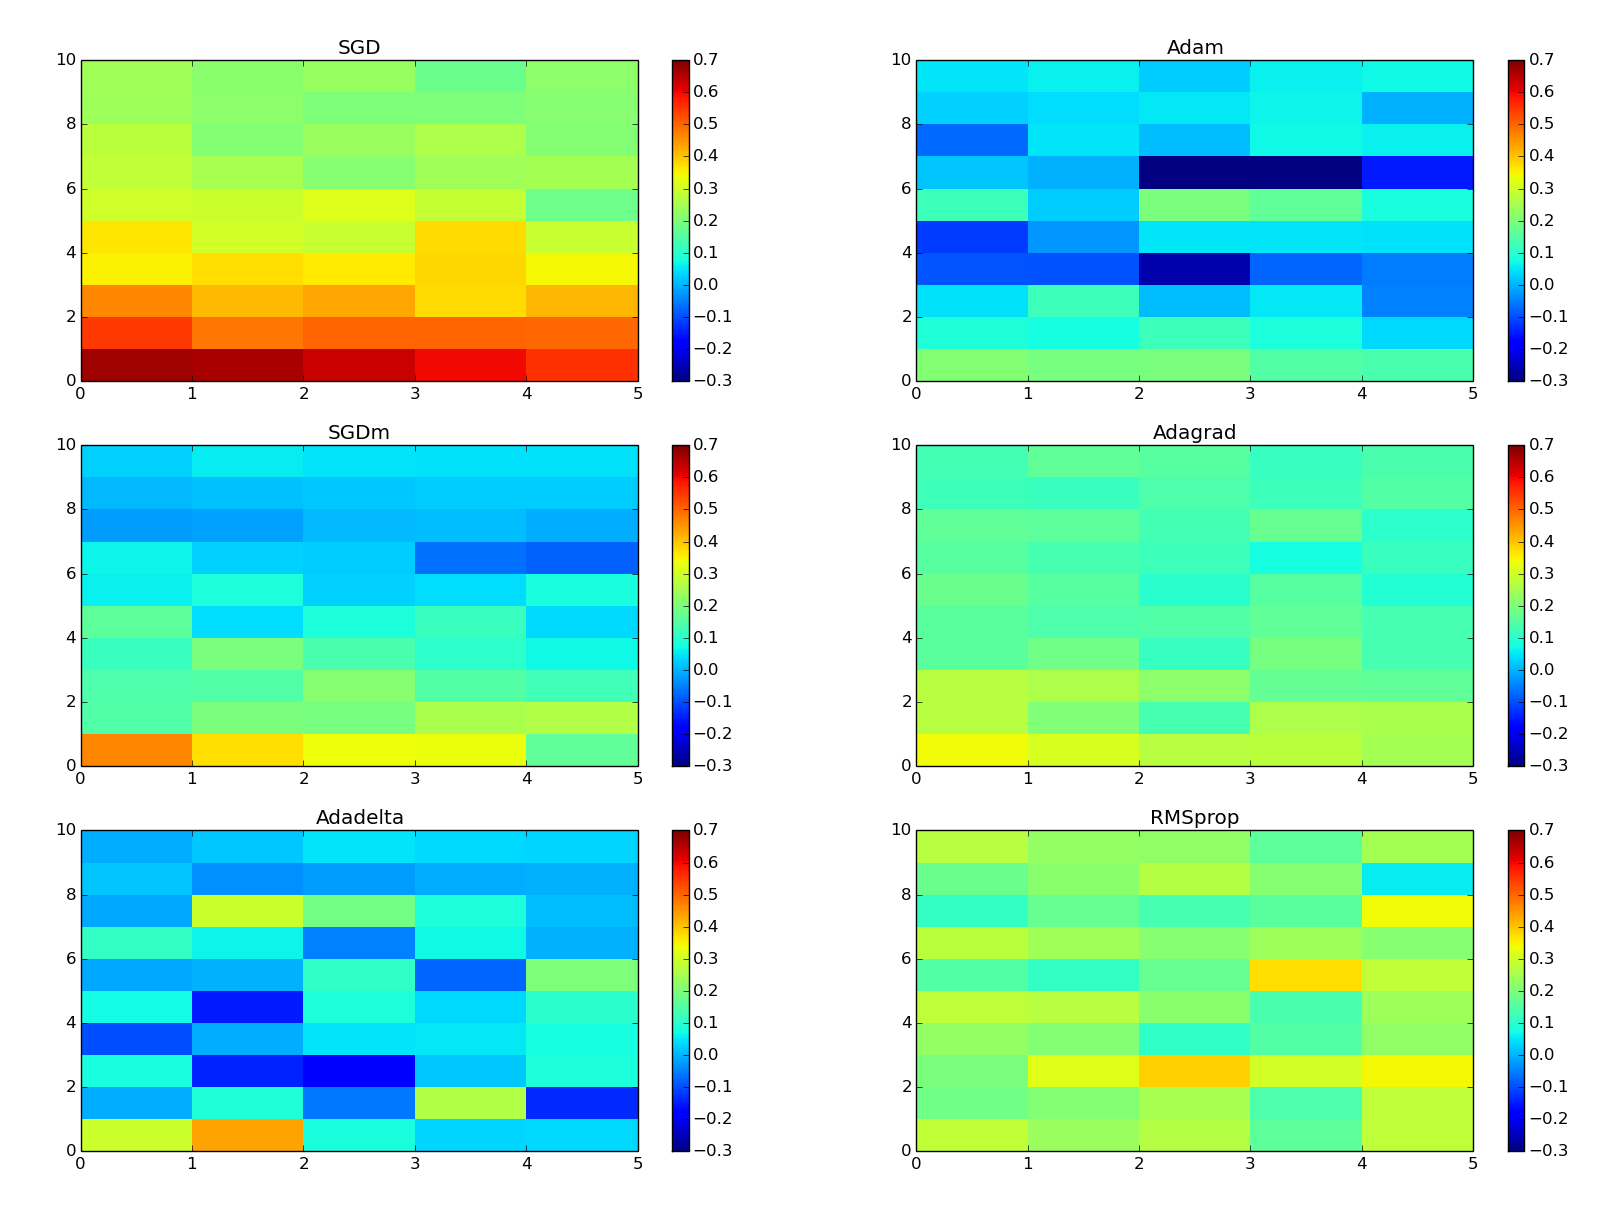
\includegraphics[scale=0.23]{map_mlp_mnist.png}
%\caption{Относительное улучшение по эпохам, MLP + MNIST}
%\end{figure}
%\end{frame}


\begin{frame}
	\frametitle{\footnotesize Качество на MNIST + MLP, топ-3 наименьшего улучшения}
\begin{table}
\centering
\scriptsize
\begin{tabular}{|c|c|c|c|c|c|}\hline
Номер эпохи & 1 & 3 & 15 & 35 & 50 \\\hline\hline
\textbf{SGD} & 89.15 & 92.84 & 96.81 & 97.58 & 97.73 \\\hline
BN SGD & 96.42 & 97.38 & 98.14 & 98.18 & 98.23 \\\hline
{Улучшение} & 0.67 & 0.63 & 0.42 & 0.25 & 0.22 \\\hline\hline
\color{red}\textbf{SGDm} & 93.39 & 96.4 & 97.83 & 98.03 & 98.03 \\\hline
BN SGDm & 96.49 & 97.62 & 98.11 & 97.87 & 98.12 \\\hline
{Улучшение} & 0.47 & 0.34 & \color{red} \textbf{0.13} & \color{red} \textbf{-0.08} & \color{red} \textbf{0.05} \\\hline\hline
\color{red}\textbf{Adam} & 93.47 & 96.03 & 97.62 & 98.04 & 98.02 \\\hline
BN Adam & 94.85 & 96.81 & 97.51 & 97.75 & 98.16 \\\hline
{Улучшение} & \color{red} \textbf{0.21} & \color{red} \textbf{0.2} & \color{red}\textbf{-0.05} & \color{red}\textbf{-0.15} & \color{red}\textbf{0.07} \\\hline\hline
\textbf{Adagrad} & 93.92 & 96.1 & 97.37 & 97.55 & 97.64 \\\hline
BN Adagrad & 96.01 & 97.16 & 97.81 & 97.84 & 97.97 \\\hline
{Улучшение} & 0.34 & 0.27 & 0.17 & 0.12 & 0.14 \\\hline\hline
\color{red}\textbf{Adadelta} & 94.28 & 96.7 & 97.51 & 98.04 & 98.2 \\\hline
BN Adadelta & 95.98 & 96.97 & 97.72 & 98.04 & 98.26 \\\hline
{Улучшение} & \color{red}\textbf{0.3} & \color{red}\textbf{0.08} & \color{red}\textbf{0.08} & \color{red}\textbf{-0.0} & \color{red}\textbf{0.03} \\\hline\hline
\textbf{RMSprop} & 94.58 & 96.14 & 96.75 & 97.34 & 97.27 \\\hline
BN RMSprop & 96.12 & 97.18 & 97.88 & 97.91 & 97.95 \\\hline
{Улучшение} & \color{red}\textbf{0.28} & \color{red}\textbf{0.27} & 0.35 & 0.21 & 0.25 \\\hline
\end{tabular}
\caption{\scriptsize Качество на MNIST + MLP, топ-3 наименьшего улучшения}
\end{table}
\end{frame}


\begin{frame}
	\frametitle{\footnotesize Качество на MNIST + MLP, топ-3 лучшего качества}
\begin{table}
\centering
\scriptsize
\begin{tabular}{|c|c|c|c|c|c|}\hline
Номер эпохи & 1 & 3 & 15 & 35 & 50 \\\hline\hline
\textbf{SGD} & 89.15 & 92.84 & 96.81 & 97.58 & 97.73 \\\hline
BN SGD & 96.42 & 97.38 & 98.14 & 98.18 & 98.23 \\\hline
{Улучшение} & 0.67 & 0.63 & 0.42 & 0.25 & 0.22 \\\hline\hline
\color{red}\textbf{SGDm} & 93.39 & \color{green} \textbf{96.4} & \color{green}\textbf{97.83} & \color{green}\textbf{98.03} & \color{green}\textbf{98.03} \\\hline
BN SGDm & 96.49 & 97.62 & 98.11 & 97.87 & 98.12 \\\hline
{Улучшение} & 0.47 & 0.34 & 0.13 & -0.08 & 0.05 \\\hline\hline
\color{red}\textbf{Adam} & 93.47 & 96.03 & \color{green}\textbf{97.62} & \color{green}\textbf{98.04} & \color{green}\textbf{98.02} \\\hline
BN Adam & 94.85 & 96.81 & 97.51 & 97.75 & 98.16 \\\hline
{Улучшение} & 0.21 & 0.2 & -0.05 & -0.15 & 0.07 \\\hline\hline
\textbf{Adagrad} & \color{green}\textbf{93.92} & 96.1 & 97.37 & 97.55 & 97.64 \\\hline
BN Adagrad & 96.01 & 97.16 & 97.81 & 97.84 & 97.97 \\\hline
{Улучшение} & 0.34 & 0.27 & 0.17 & 0.12 & 0.14 \\\hline\hline
\color{red}\textbf{Adadelta} & \color{green}\textbf{94.28} & \color{green}\textbf{96.7} & \color{green}\textbf{97.51} & \color{green}\textbf{98.04} & \color{green}\textbf{98.2} \\\hline
BN Adadelta & 95.98 & 96.97 & 97.72 & 98.04 & 98.26 \\\hline
{Улучшение} & 0.3 & 0.08 & 0.08 & -0.0 & 0.03 \\\hline\hline
\textbf{RMSprop} & \color{green}\textbf{94.58} & \color{green}\textbf{96.14} & 96.75 & 97.34 & 97.27 \\\hline
BN RMSprop & 96.12 & 97.18 & 97.88 & 97.91 & 97.95 \\\hline
{Улучшение} & 0.28 & 0.27 & 0.35 & 0.21 & 0.25 \\\hline
\end{tabular}
\caption{\scriptsize Качество на MNIST + MLP, топ-3 лучшего качества}
\end{table}
\end{frame}

%\begin{frame}
%	\frametitle{Эксперименты: численные результаты}
%\begin{table}
%\centering
%\scriptsize
%\begin{tabular}{|c|c|c|c|c|c|c|c|c|}\hline
%Номер эпохи & 1 & 2 & 3 & 15 & 35 & 50 \\\hline
%SGD & 89.15 & 91.87 & 92.84 & 96.81 & 97.58 & 97.73 \\\hline
%BN SGD & 96.42 & 97.27 & 97.38 & 98.14 & 98.18 & 98.23 \\\hline
%\textbf{Улучшение} & 0.67 & 0.66 & 0.63 & 0.42 & 0.25 & 0.22 \\\hline
%SGDm & 93.39 & 95.55 & 96.4 & 97.83 & 98.03 & 98.03 \\\hline
%BN SGDm & 96.49 & 97.22 & 97.62 & 98.11 & 97.87 & 98.12 \\\hline
%\textbf{Улучшение} & 0.47 & 0.38 & 0.34 & 0.13 & -0.08 & 0.05 \\\hline
%Adam & 93.47 & 95.48 & 96.03 & 97.62 & 98.04 & 98.02 \\\hline
%BN Adam & 94.85 & 96.35 & 96.81 & 97.51 & 97.75 & 98.16 \\\hline
%\textbf{Улучшение} & 0.21 & 0.19 & 0.2 & -0.05 & -0.15 & 0.07 \\\hline
%Adagrad & 93.92 & 95.61 & 96.1 & 97.37 & 97.55 & 97.64 \\\hline
%BN Adagrad & 96.01 & 96.98 & 97.16 & 97.81 & 97.84 & 97.97 \\\hline
%\textbf{Улучшение} & 0.34 & 0.31 & 0.27 & 0.17 & 0.12 & 0.14 \\\hline
%Adadelta & 94.28 & 94.3 & 96.7 & 97.51 & 98.04 & 98.2 \\\hline
%BN Adadelta & 95.98 & 96.78 & 96.97 & 97.72 & 98.04 & 98.26 \\\hline
%\textbf{Улучшение} & 0.3 & 0.44 & 0.08 & 0.08 & -0.0 & 0.03 \\\hline
%RMSprop & 94.58 & 96.17 & 96.14 & 96.75 & 97.34 & 97.27 \\\hline
%BN RMSprop & 96.12 & 97.08 & 97.18 & 97.88 & 97.91 & 97.95 \\\hline
%\textbf{Улучшение} & 0.28 & 0.24 & 0.27 & 0.35 & 0.21 & 0.25 \\\hline
%\end{tabular}
%\caption{\scriptsize Качество на MNIST + MLP, лучшие рейты}
%\end{table}
%\end{frame}

%\begin{frame}
%	\frametitle{Результаты}
%*еще одна тепловая карта другого типа, для CNN + CIFAR-10
%\end{frame}

\begin{frame}
	\frametitle{\footnotesize Качество на CIFAR-10 + CNN, топ-3 наименьшего улучшения}
\begin{table}
\centering
\scriptsize
\begin{tabular}{|c|c|c|c|c|c|}\hline
Номер эпохи & 1 & 2 & 25 & 35 & 50 \\\hline\hline
\textbf{SGD} & 24.26 & 22.14 & 58.95 & 63.23 & 65.45 \\\hline
BN SGD & 48.47 & 52.95 & 71.31 & 75.89 & 76.58 \\\hline
{Улучшение} & 0.32 & 0.4 & 0.3 & 0.34 & 0.32 \\\hline\hline
\textbf{SGDm} & 30.03 & 37.98 & 64.37 & 68.3 & 71.54 \\\hline
BN SGDm & 53.72 & 58.76 & 76.85 & 76.89 & 78.39 \\\hline
{Улучшение} & 0.34 & 0.34 & 0.35 & 0.27 & 0.24 \\\hline\hline
\color{red}\textbf{Adam} & 43.28 & 47.3 & 68.02 & 70.79 & 72.54 \\\hline
BN Adam & 53.94 & 59.13 & 75.4 & 76.63 & 76.66 \\\hline
{Улучшение} & \color{red}\textbf{0.19} & \color{red}\textbf{0.22} & \color{red}\textbf{0.23} &\color{red}\textbf{ 0.2} & \color{red}\textbf{0.15} \\\hline\hline
\textbf{Adagrad} & 29.82 & 37.25 & 60.86 & 62.35 & 64.63 \\\hline
BN Adagrad & 48.24 & 53.83 & 74.66 & 76.11 & 76.96 \\\hline
{Улучшение} & \color{red}\textbf{0.26} & \color{red}\textbf{0.26} & 0.35 & 0.37 & 0.35 \\\hline\hline
\color{red}\textbf{Adadelta} & 31.31 & 32.96 & 67.12 & 70.56 & 70.81 \\\hline
BN Adadelta & 49.62 & 55.96 & 72.75 & 76.99 & 77.2 \\\hline
{Улучшение} & 0.27 & 0.34 & \color{red}\textbf{0.17} & \color{red}\textbf{0.22} & \color{red}\textbf{0.22} \\\hline\hline
\color{red}\textbf{RMSprop} & 25.6 & 39.89 & 64.24 & 68.96 & 70.31 \\\hline
BN RMSprop & 42.61 & 52.98 & 73.7 & 75.47 & 75.81 \\\hline
{Улучшение} & \color{red}\textbf{0.23} & \color{red}\textbf{0.22} & \color{red}\textbf{0.26} & \color{red}\textbf{0.21} & \color{red}\textbf{0.19} \\\hline
\end{tabular}
\caption{\scriptsize Качество на CIFAR-10 + CNN, топ-3 наименьшего улучшения}
\end{table}
\end{frame}

\begin{frame}
	\frametitle{\footnotesize Качество на CIFAR-10 + CNN, топ-3 лучшего качества}
\begin{table}
\centering
\scriptsize
\begin{tabular}{|c|c|c|c|c|c|}\hline
Номер эпохи & 1 & 2 & 25 & 35 & 50 \\\hline \hline
\textbf{SGD} & 24.26 & 22.14 & 58.95 & 63.23 & 65.45 \\\hline
BN SGD & 48.47 & 52.95 & 71.31 & 75.89 & 76.58 \\\hline
Улучшение & 0.32 & 0.4 & 0.3 & 0.34 & 0.32 \\\hline\hline
\textbf{SGDm} & \color{green}\textbf{30.03} & \color{green}\textbf{37.98} & \color{green}\textbf{64.37} & 68.3 & \color{green}\textbf{71.54} \\\hline 
BN SGDm & 53.72 & 58.76 & 76.85 & 76.89 & 78.39 \\\hline
Улучшение & 0.34 & 0.34 & 0.35 & 0.27 & 0.24 \\\hline\hline
\color{red}\textbf{Adam} & \color{green}\textbf{43.28} &\color{green}\textbf{47.3} & \color{green}\textbf{68.02} & \color{green}\textbf{70.79} & \color{green}\textbf{72.54} \\\hline
BN Adam & 53.94 & 59.13 & 75.4 & 76.63 & 76.66 \\\hline
Улучшение & 0.19 & 0.22 & 0.23 & 0.2 & 0.15 \\\hline\hline
\textbf{Adagrad} & 29.82 & 37.25 & 60.86 & 62.35 & 64.63 \\\hline
BN Adagrad & 48.24 & 53.83 & 74.66 & 76.11 & 76.96 \\\hline
Улучшение & 0.26 & 0.26 & 0.35 & 0.37 & 0.35 \\\hline\hline
\color{red}\textbf{Adadelta} & \color{green}\textbf{31.31} & 32.96 & \color{green}\textbf{67.12} & \color{green}\textbf{70.56} & \color{green}\textbf{70.81} \\\hline
BN Adadelta & 49.62 & 55.96 & 72.75 & 76.99 & 77.2 \\\hline
Улучшение & 0.27 & 0.34 & 0.17 & 0.22 & 0.22 \\\hline\hline
\color{red}\textbf{RMSprop} & 25.6 & \color{green}\textbf{39.89} & 64.24 & \color{green}\textbf{68.96} & 70.31 \\\hline
BN RMSprop & 42.61 & 52.98 & 73.7 & 75.47 & 75.81 \\\hline
Улучшение & 0.23 & 0.22 & 0.26 & 0.21 & 0.19 \\\hline
\end{tabular}
\caption{\scriptsize Качество на CIFAR-10 + CNN, топ-3 лучшего качества}
\end{table}
\end{frame}

\section{Выводы}

\begin{frame}
	\frametitle{Выводы}
\begin{itemize}
\item Батч-нормализация тем слабее улучшает метод, чем он сам по себе качественнее работает
\item Возможно, батч-нормализация плохо совместима с инерцией для полносвязных сетей
\item Возможно, батч-нормализация плохо совместима с методами, наследуемыми от RMSprop, для сверточных сетей
%\item Эксперименты по сравнению дисперсии градиента для инерции и батч-нормализации?
%\item Батч-нормализация плохо комбинируется с Адамом. Эксперименты?
\end{itemize}
\end{frame}



\begin{frame}
\frametitle{На защиту выносится:}
\begin{enumerate}
\item Реализация двух архитектур нейронной сети с батч нормализацией и пяти модификаций стохастического градиентного спуска
\item Экспериментальные исследования модификаций стохастического градиентного спуска для обучения нейронных сетей с и без батч-нормализации
\item ?Рекомендации по использованию батч-нормализации и модификаций стохастического градиентного спуска при обучении нейронных сетей
\end{enumerate}
\end{frame}

\begin{frame}
	\frametitle{Конец}
\begin{center}
Конец!
\end{center}

\end{frame}



\begin{frame}
\frametitle{SGD}
\[\theta_{t+1} = \theta_t - \eta \nabla F(\theta)\]	
\end{frame}

\begin{frame}
\frametitle{SGD momentum}
\[v_{t+1} = \mu v_t - \eta \nabla F(\theta)\]
\[\theta_{t+1} = \theta_t + v_{t+1}\]	
\end{frame}

\begin{frame}
\frametitle{Adagrad}
\[g_{t+1} = g_t + \nabla F(\theta) ^2\]
\[\theta_{t+1} = \theta_t - \frac{\eta \nabla F(\theta)}{\sqrt{g_{t+1}} + \epsilon}\]	
\end{frame}

\begin{frame}
\frametitle{RMSprop}
\[g_{t+1} = \gamma g_t + (1 - \gamma) \nabla F(\theta)^2\]
\[\theta_{t+1} = \theta_t - \frac{\eta \nabla F(\theta)}{\sqrt{g_{t+1} + \epsilon}}\]	
\end{frame}

\begin{frame}
\frametitle{Adadelta}
\[g_{t+1} = \gamma g_t + (1 - \gamma) \nabla F(\theta)^2\]
\[v_{t+1} = - \frac{\sqrt{x_t + \epsilon} \nabla F(\theta)}{\sqrt{g_{t+1} + \epsilon}}\]
\[x_{t+1} = \gamma x_t + (1 - \gamma) v_{t+1}^2\]
\[\theta_{t+1} = \theta_t + v_{t+1}\]	
\end{frame}

\begin{frame}
\frametitle{Adam}
\[m_{t+1} = \gamma_1 m_t + (1 - \gamma_1) \nabla F(\theta)\]
\[g_{t+1} = \gamma_2 g_t + (1 - \gamma_2) \nabla F(\theta)^2\]
\[\hat{m}_{t+1} = \frac{m_{t+1}}{1 - \gamma_1^{t+1}}\]
\[\hat{g}_{t+1} = \frac{m_{t+1}}{1 - \gamma_2^{t+1}}\]
\[\theta_{t+1} = \theta_t - \frac{\eta \hat{m}_{t+1}}{\sqrt{\hat{g}_{t+1}} + \epsilon}\]	
\end{frame}

	
\end{document}
